\documentclass[12pt]{beamer}
\usepackage{Estilos/BeamerFC}
\usepackage{Estilos/ColoresLatex}
\usetheme{Warsaw}
\usecolortheme{seahorse}
%\useoutertheme{default}
\setbeamercovered{invisible}
% or whatever (possibly just delete it)
\setbeamertemplate{section in toc}[sections numbered]
\setbeamertemplate{subsection in toc}[subsections numbered]
\setbeamertemplate{subsection in toc}{\leavevmode\leftskip=3.2em\rlap{\hskip-2em\inserttocsectionnumber.\inserttocsubsectionnumber}\inserttocsubsection\par}
\setbeamercolor{section in toc}{fg=blue}
\setbeamercolor{subsection in toc}{fg=blue}
\setbeamercolor{frametitle}{fg=blue}
\setbeamertemplate{caption}[numbered]

\setbeamertemplate{footline}
\beamertemplatenavigationsymbolsempty
\setbeamertemplate{headline}{}


\makeatletter
\setbeamercolor{section in foot}{bg=gray!30, fg=black!90!orange}
\setbeamercolor{subsection in foot}{bg=blue!30}
\setbeamercolor{date in foot}{bg=black}
\setbeamertemplate{footline}
{
  \leavevmode%
  \hbox{%
  \begin{beamercolorbox}[wd=.333333\paperwidth,ht=2.25ex,dp=1ex,center]{section in foot}%
    \usebeamerfont{section in foot} \insertsection
  \end{beamercolorbox}%
  \begin{beamercolorbox}[wd=.333333\paperwidth,ht=2.25ex,dp=1ex,center]{subsection in foot}%
    \usebeamerfont{subsection in foot}  \insertsubsection
  \end{beamercolorbox}%
  \begin{beamercolorbox}[wd=.333333\paperwidth,ht=2.25ex,dp=1ex,right]{date in head/foot}%
    \usebeamerfont{date in head/foot} {T1 - Segunda presentación} \hspace*{2em}
    \insertframenumber{} / \inserttotalframenumber \hspace*{2ex} 
  \end{beamercolorbox}}%
  \vskip0pt%
}
\makeatother

\makeatletter
\patchcmd{\beamer@sectionintoc}{\vskip1.5em}{\vskip0.8em}{}{}
\makeatother
\usepackage{pifont}
\newcommand{\cmark}{\ding{51}}%
\newcommand{\xmark}{\ding{55}}%

\makeatletter
\setbeamertemplate{footline}
{
  \leavevmode%
  \hbox{%
  \begin{beamercolorbox}[wd=.333333\paperwidth,ht=2.25ex,dp=1ex,center]{section in foot}%
    \usebeamerfont{section in foot} \insertsection
  \end{beamercolorbox}%
  \begin{beamercolorbox}[wd=.333333\paperwidth,ht=2.25ex,dp=1ex,center]{subsection in foot}%
    \usebeamerfont{subsection in foot}  \insertsubsection
  \end{beamercolorbox}%
  \begin{beamercolorbox}[wd=.333333\paperwidth,ht=2.25ex,dp=1ex,right]{date in head/foot}%
    \usebeamerfont{date in head/foot} \insertshortdate{} \hspace*{2em}
    \insertframenumber{} / \inserttotalframenumber \hspace*{2ex} 
  \end{beamercolorbox}}%
  \vskip0pt%
}
\makeatother

\setbeamertemplate{navigation symbols}{}
\date{1 de abril de 2023}

\title{Los vectores en la física}
\subtitle{Curso de Física I}

\begin{document}

\maketitle
\fontsize{14}{14}\selectfont
\spanishdecimal{.}

\section*{Contenido}
\frame[allowframebreaks]{\frametitle{Puntos a revisar}\tableofcontents[currentsection, hideallsubsections]}

\section{Vectores}
\frame{\frametitle{Contenido}\tableofcontents[currentsection, hideothersubsections]}
\subsection{Definición}

\begin{frame}
\frametitle{¿Qué es un vector?}
Los vectores se definen como expresiones matemáticas que poseen magnitud, dirección y sentido.
\\
\bigskip
\pause
Los vectores se representan por flechas en las ilustraciones, normalmente se distinguen de las cantidades escalares mediante el uso de negritas ($\vb{P}$).
\end{frame}
\begin{frame}
\frametitle{Varios vectores}
\begin{figure}
    \centering
    \begin{tikzpicture}
        \draw [-stealth, thick] (0, 0) -- (3, 2) node [midway, above] {$\va{P}$};
        \draw (0, 0) -- (2, 0);
        \draw (0.5, 0) arc(0:30:0.6);
        \node at (0.8, 0.2) {$\theta$}; \pause
        \draw [stealth-, thick] (7, 1) -- (9, 1) node [midway, above] {$\va{A}$};
    \end{tikzpicture}
\end{figure}
\end{frame}
\begin{frame}
\frametitle{Escribiendo vectores}
En la escritura a mano, un vector puede caracterizarse dibujando una pequeña flecha arriba de la letra usada para representarlo ($\va{P}$).
\\
\bigskip
\pause
La magnitud de un vector determina la longitud de la flecha correspondiente.
\end{frame}
\begin{frame}
\frametitle{Definiendo un vector}
\begin{figure}
    \centering
    \begin{tikzpicture}
        \draw [-stealth, thick] (0, 0) -- (3, 3) node [midway, above] {$\va{P}$};
        \draw [dashed] (-1, -1) -- (4, 4); 
        \draw (0, 0) -- (2, 0);
        \draw (0.5, 0) arc(0:30:0.8);
        \node at (0.8, 0.2) {$\theta$};
        \node at (5, 4) {Línea de acción};
    \end{tikzpicture}
\end{figure}
\end{frame}
\begin{frame}
\frametitle{Dirección de un vector}
La dirección de un vector representa el ángulo de inclinación con respecto a una línea horizontal medidad en el sentido antihorario.
\pause
\begin{figure}
    \centering
    \begin{tikzpicture}
        \draw [-stealth, thick] (0, 0) -- (2, 2) node [midway, above] {$\va{A}$};
        \draw [dashed] (-0.5, -0.5) -- (2.5, 2.5); 
        \draw (0, 0) -- (2, 0);
        \draw (0.5, 0) arc(0:45:0.5);
        \node at (1.5, 0.2) {$\theta = \ang{45}$};
        
        \pause
        
        \draw [-stealth, thick] (6, 0) -- (4, 2) node [midway, above] {$\va{B}$};
        \draw [dashed] (7, -1) -- (3, 3); 
        \draw (6, 0) -- (8.5, 0);
        \draw (6.5, 0) arc(0:135:0.55);
        \node at (7.5, 0.2) {$\theta = \ang{135}$};
    \end{tikzpicture}
\end{figure}
\end{frame}

\subsection{Tipos de vectores}

\begin{frame}
\frametitle{Vectores colineales}
Son aquellos que están contenidos en una misma línea de acción.
\pause
\begin{figure}
    \centering
    \begin{tikzpicture}
        \draw [dashed] (0, 0) -- (10, 0);
        \draw [-stealth, thick] (1, 0) -- (2, 0) node [above, midway] {$\va{A}$};
        \draw [stealth-, thick] (4, 0) -- (5, 0) node [above, midway] {$\va{B}$};
        \draw [-stealth, thick] (7, 0) -- (8, 0) node [above, midway] {$\va{C}$};
    \end{tikzpicture}
\end{figure}
\end{frame}
\begin{frame}
\frametitle{Vectores concurrentes}
Son aquellos cuyas líneas de acción se cortan en un mismo punto.
\pause
\begin{figure}
    \centering
    \begin{tikzpicture}
        \draw [dashed] (0, 0) -- (6, 0);
        \draw [-stealth, thick] (1, 0) -- (2, 0) node [above, midway] {$\va{A}$};
        \draw [stealth-, thick] (5, 0) -- (6, 0) node [above, midway] {$\va{B}$};
        
        \draw [dashed] (3, 3) -- (3, -2);
        \draw [-stealth, thick] (3, 3) -- (3, 2) node [left, midway] {$\va{C}$};
    \end{tikzpicture}
\end{figure}
\end{frame}
\begin{frame}
\frametitle{Vectores coplanares}
Son aquellos que se encuentran en un mismo plano:
\pause
\begin{figure}
    \centering
    \begin{tikzpicture}
        \draw[fill=aquamarine] (0, 0) rectangle (5, 3);
        \draw [-stealth, thick] (0.5, 1) -- (1.5, 1) node [above, midway] {$\va{a}$};
        \draw [-stealth, thick] (4, 2) -- (3, 1) node [above, midway] {$\va{b}$};
        \draw [-stealth, thick] (2.5, 1) -- (2.5, 2) node [left, midway] {$\va{c}$};
    \end{tikzpicture}
\end{figure}
\end{frame}

\section{Operaciones con vectores}
\frame{\frametitle{Contenido}\tableofcontents[currentsection, hideothersubsections]}
\subsection{Suma de vectores}

\begin{frame}
\frametitle{El método del paralelogramo}
Por definición, los vectores se suman de acuerdo con la \emph{ley del paralelogramo}.
\\
\bigskip
\pause
Así, la suma de dos vectores $\va{P}$ y $\va{Q}$ se obtiene uniendo los dos vectores al mismo punto $A$ y construyendo un paralelogramo que tenga por lados a $\va{P}$ y a $\va{Q}$.
\end{frame}
\begin{frame}
\frametitle{El método del paralelogramo}
\begin{figure}
    \centering
    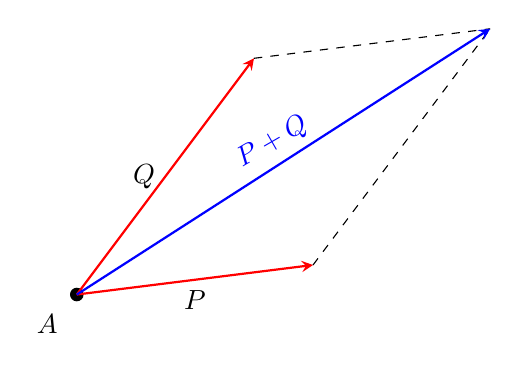
\begin{tikzpicture}[scale=1.5]
        \draw [fill] (0, 0) circle (1.5pt);
        \node at (-0.25, -0.25) {$A$};
        \draw [-stealth, thick, color=red, text=black] (0, 0) -- (2, 0.25) node [below, midway] {$\va{P}$};
        \draw [-stealth, thick, color=red, text=black] (0, 0) -- (1.5, 2) node [left, midway] {$\va{Q}$}; \pause
        \draw [dashed] (2, 0.25) -- (3.5, 2.25); \pause
        \draw [dashed] (1.5, 2) -- (3.5, 2.25); \pause
        \draw [-stealth, thick, color=blue] (0, 0) -- (3.5, 2.25) node [above, midway, rotate=30] {$\va{P} + \va{Q}$};
    \end{tikzpicture}
\end{figure}
\end{frame}
\begin{frame}
\frametitle{El vector resultante}
La diagonal que pasa por $A$ representa la suma vectorial de $\va{P}$ y $\va{Q}$, y se representa por $\va{P} + \va{Q}$.
\end{frame}
\begin{frame}
\frametitle{La regla del triángulo}
A partir de la ley del paralelogramo se puede obtener otro método para determinar
la suma de dos vectores.
\end{frame}
\begin{frame}
\frametitle{La regla del triángulo}    
Este método, llamado \textocolor{ao}{regla del triángulo}, se obtiene como sigue: \pause nos apoyamos con la siguiente figura:
\end{frame}
\begin{frame}
\frametitle{La regla del triángulo}    
\begin{figure}
    \centering
    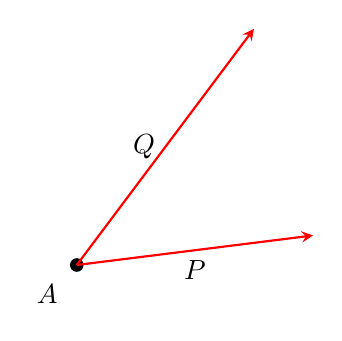
\begin{tikzpicture}[scale=1.5]
        \draw [fill] (0, 0) circle (1.5pt);
        \node at (-0.25, -0.25) {$A$};
        \draw [-stealth, thick, color=red, text=black] (0, 0) -- (2, 0.25) node [below, midway] {$\va{P}$};
        \draw [-stealth, thick, color=red, text=black] (0, 0) -- (1.5, 2) node [left, midway] {$\va{Q}$};
        % \draw [dashed] (2, 0.25) -- (3.5, 2.25); \pause
        % \draw [dashed] (1.5, 2) -- (3.5, 2.25); \pause
        % \draw [-stealth, thick, color=blue] (0, 0) -- (3.5, 2.25) node [above, midway, rotate=30] {$\va{P} + \va{Q}$};
    \end{tikzpicture}
\end{figure}
\end{frame}
\begin{frame}
\frametitle{La regla del triángulo}    
\begin{figure}
    \centering
    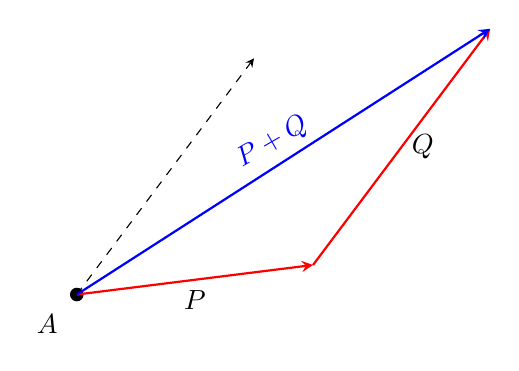
\begin{tikzpicture}[scale=1.5]
        \draw [fill] (0, 0) circle (1.5pt);
        \node at (-0.25, -0.25) {$A$};
        \draw [-stealth, thick, color=red, text=black] (0, 0) -- (2, 0.25) node [below, midway] {$\va{P}$}; \pause
        \draw [-stealth, dashed] (0, 0) -- (1.5, 2);
        \draw [-stealth, thick, color=red, text=black] (2, 0.25) -- (3.5, 2.25) node [right, midway] {$\va{Q}$}; \pause
        \draw [-stealth, thick, color=blue] (0, 0) -- (3.5, 2.25) node [above, midway, rotate=30] {$\va{P} + \va{Q}$};
    \end{tikzpicture}
\end{figure}
\end{frame}
\begin{frame}
\frametitle{La ley de triángulo}
La suma de los dos vectores puede encontrarse colocando $\va{P}$ y $\va{Q}$ de punta a cola y uniendo la cola de $\va{P}$ con la punta de $\va{Q}$.
\end{frame}
\begin{frame}
\frametitle{La regla del triángulo}    
\begin{figure}
    \centering
    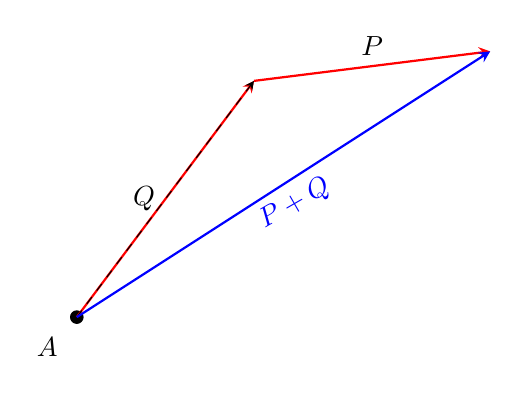
\begin{tikzpicture}[scale=1.5]
        \draw [fill] (0, 0) circle (1.5pt);
        \node at (-0.25, -0.25) {$A$};
        \draw [-stealth, thick, color=red, text=black] (0, 0) -- (1.5, 2) node [left, midway] {$\va{Q}$}; \pause
        \draw [-stealth, thick, color=red, text=black] (1.5, 2) -- (3.5, 2.25) node [above, midway] {$\va{P}$}; \pause
        \draw [-stealth, dashed] (0, 0) -- (1.5, 2);
        \draw [-stealth, thick, color=blue] (0, 0) -- (3.5, 2.25) node [below, midway, rotate=30] {$\va{P} + \va{Q}$};
    \end{tikzpicture}
\end{figure}
\end{frame}
\begin{frame}
\frametitle{La suma con más vectores}
La suma de tres vectores $\va{P}$, $\va{Q}$ y $\va{S}$ se obtiene, por definición, sumando primero los vectores $\va{P}$ y $\va{Q}$ y agregando el vector $\va{S}$ al vector $\va{P} + \va{Q}$:
\end{frame}
\begin{frame}
\frametitle{La regla del triángulo}    
\begin{figure}
    \centering
    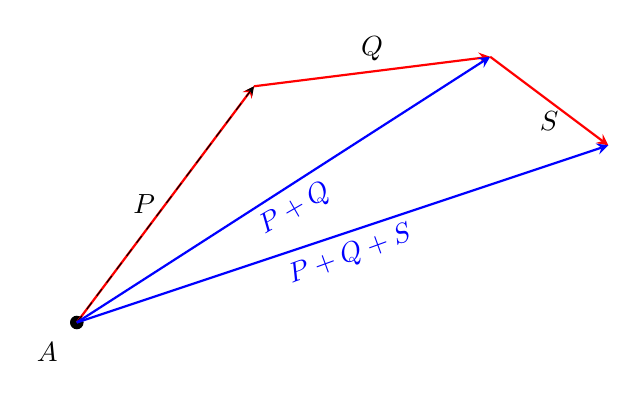
\begin{tikzpicture}[scale=1.5]
        \draw [fill] (0, 0) circle (1.5pt);
        \node at (-0.25, -0.25) {$A$};
        \draw [-stealth, thick, color=red, text=black] (0, 0) -- (1.5, 2) node [left, midway] {$\va{P}$}; \pause
        \draw [-stealth, thick, color=red, text=black] (1.5, 2) -- (3.5, 2.25) node [above, midway] {$\va{Q}$}; \pause
        \draw [-stealth, dashed] (0, 0) -- (1.5, 2);
        \draw [-stealth, thick, color=blue] (0, 0) -- (3.5, 2.25) node [below, midway, rotate=30] {$\va{P} + \va{Q}$}; \pause
        \draw [-stealth, thick, color=red, text=black] (3.5, 2.25) -- (4.5, 1.5) node [below, midway] {$\va{S}$}; \pause
        \draw [-stealth, thick, color=blue] (0, 0) -- (4.5, 1.5) node [below, midway, rotate=20] {$\va{P} + \va{Q} + \va{S}$};
    \end{tikzpicture}
\end{figure}
\end{frame}

\section{Ejercicios}
\frame{\frametitle{Contenido}\tableofcontents[currentsection, hideothersubsections]}
\subsection{Ejercicio 1}

\begin{frame}
\frametitle{Enunciado del Ejercicio 1}
En una competencia, un corredor realiza los siguientes desplazamientos:
\setbeamercolor{item projected}{bg=bananayellow,fg=blue}
\setbeamertemplate{enumerate items}{%
\usebeamercolor[bg]{item projected}%
\raisebox{1.5pt}{\colorbox{bg}{\color{fg}\footnotesize\insertenumlabel}}%
}
\begin{enumerate}[<+->]
\item $d_{1} = \SI{400}{\meter}, \theta = \ang{35}$
\item $d_{2} = \SI{700}{\meter}, \theta = \ang{120}$
\item $d_{3} = \SI{600}{\meter}, \theta = \ang{190}$
\item $d_{4} = \SI{200}{\meter}, \theta = \ang{250}$
\end{enumerate}
\end{frame}
\begin{frame}
\frametitle{Enunciado del ejercicio 1}
Encuentra gráficamente cuál es el desplazamiento resultante del corredor y cuál es el valor del ángulo del desplazamiento resultante, medido respecto al eje $x$ positivo.
\end{frame}
\begin{frame}
\frametitle{Solución al Ejercicio 1}
Utilizando el método gráfico \enquote{conectamos} los vectores con la correspondiente orientación que se indica con el ángulo de cada uno de ellos.
\end{frame}
\begin{frame}[plain]
\begin{figure}
    \centering
    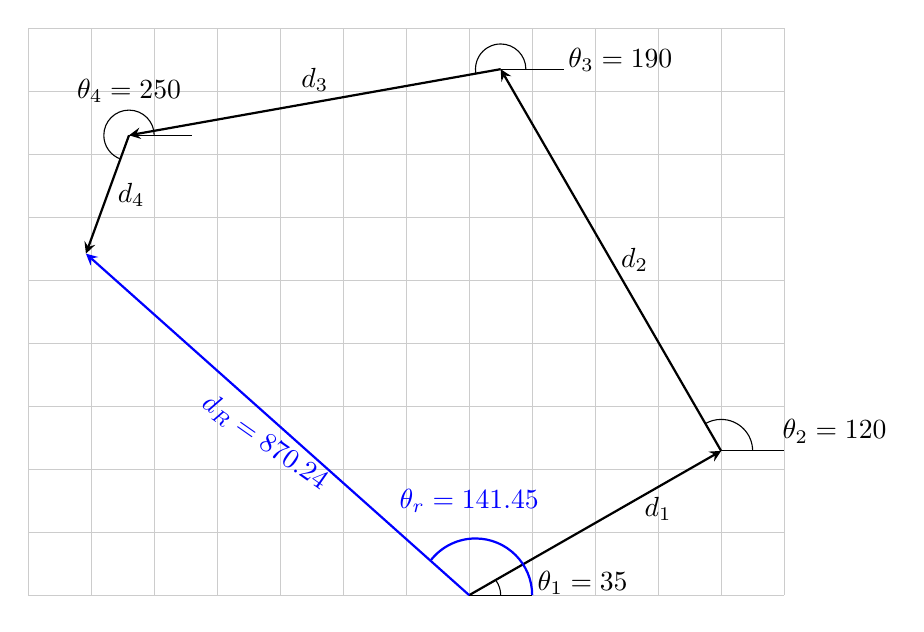
\begin{tikzpicture}[scale=0.8]
        \draw[thin, gray!40] (-7, 0) grid (5, 9);
        \draw [-stealth, thick] (0, 0) -- (4, 2.29) node [below, near end] {$d_{1}$};
        \draw (0, 0) -- (1, 0);
        \draw (0.5, 0) arc(0:35:0.4);
        \node at (1.8, 0.2) {$\theta_{1} = \ang{35}$};
        \pause
        \draw [-stealth, thick] (4, 2.29) -- (0.5, 8.35) node [midway, right] {$d_{2}$};
        \draw (4, 2.29) -- (5, 2.29);
        \draw (4.5, 2.29) arc(0:120:0.5);
        \node at (5.8, 2.6) {$\theta_{2} = \ang{120}$};
        \pause
        \draw [-stealth, thick] (0.5, 8.35) -- (-5.4, 7.3) node [above, midway] {$d_{3}$};
        \draw (0.5, 8.35) -- (1.5, 8.35);
        \draw (0.9, 8.35) arc(0:190:0.4);
        \node at (2.4, 8.5) {$\theta_{3} = \ang{190}$};
        \pause
        \draw [-stealth, thick] (-5.4, 7.3) -- (-6.084, 5.421) node [midway, right] {$d_{4}$};
        \draw (-5.4, 7.3) -- (-4.4, 7.3);
        \draw (-5, 7.3) arc(0:250:0.4);
        \node at (-5.4, 8) {$\theta_{4} = \ang{250}$};
        \pause
        \draw [-stealth, thick, color=blue] (0, 0) -- (-6.084, 5.421) node [midway, below, rotate=-35] {$d_{R} = \SI{870.24}{\meter}$}; \pause
        \draw [thick, color=blue] (1, 0) arc(0:141.45:0.9);
        \node [blue] at (0, 1.5) {$\theta_{r} = \ang{141.45}$};
    \end{tikzpicture}
\end{figure}
\end{frame}

\subsection{Método analítico}

\begin{frame}
\frametitle{Descomposición en componentes}
Es sabido que todo vector $\va{A}$ se puede \enquote{descomponer} en las llamadas \emph{componentes}, tanto en la dirección del eje $x$, como del eje $y$. 
\end{frame}
\begin{frame}
\frametitle{Base geométrica}
Para obtener las componentes del vector, recordemos de la geometría, el caso de un triángulo rectángulo: \pause
\begin{figure}
    \centering
    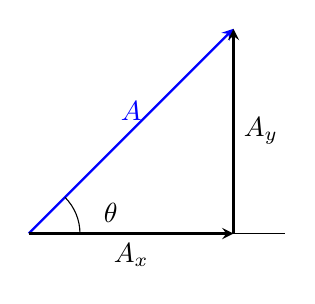
\begin{tikzpicture}[scale=1.3]
        \draw [-stealth, thick, color=blue] (0, 0) -- (2, 2) node [above, midway] {$\va{A}$};
        \draw (0.5, 0) arc(0:45:0.5);
        \node at (0.8, 0.2) {$\theta$};
        \draw (0, 0) -- (2.5, 0); \pause
        \draw [-stealth, thick] (2, 0) -- (2, 2) node [right, midway] {$A_{y}$}; \pause
        \draw [-stealth, thick] (0, 0) -- (2, 0) node [below, midway] {$A_{x}$};
    \end{tikzpicture}
\end{figure}
\end{frame}
\begin{frame}
\frametitle{Base geométrica}
\begin{figure}
    \centering
    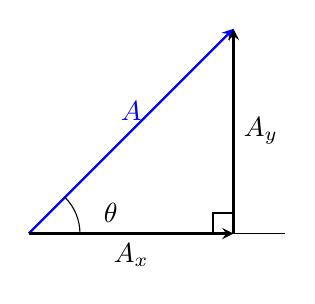
\begin{tikzpicture}[scale=1.3]
        \draw [-stealth, thick, color=blue] (0, 0) -- (2, 2) node [above, midway] {$\va{A}$};
        \draw (0.5, 0) arc(0:45:0.5);
        \node at (0.8, 0.2) {$\theta$};
        \draw (0, 0) -- (2.5, 0);
        \draw [-stealth, thick] (2, 0) -- (2, 2) node [right, midway] {$A_{y}$};
        \draw [-stealth, thick] (0, 0) -- (2, 0) node [below, midway] {$A_{x}$};
        \draw (1.8, 0) -- (1.8, 0.2) -- (2, 0.2);
    \end{tikzpicture}
\end{figure}
Las componentes del vector son:
\begin{eqnarray*}
\begin{aligned}
A_{x} &= \cos \theta \, \abs{A} \\[0.5em] \pause
A_{y} &= \sin \theta \, \abs{A}
\end{aligned}
\end{eqnarray*}
\end{frame}
\begin{frame}
\frametitle{Base geométrica}
\begin{figure}
    \centering
    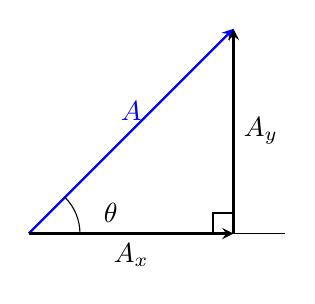
\begin{tikzpicture}[scale=1.3]
        \draw [-stealth, thick, color=blue] (0, 0) -- (2, 2) node [above, midway] {$\va{A}$};
        \draw (0.5, 0) arc(0:45:0.5);
        \node at (0.8, 0.2) {$\theta$};
        \draw (0, 0) -- (2.5, 0);
        \draw [-stealth, thick] (2, 0) -- (2, 2) node [right, midway] {$A_{y}$};
        \draw [-stealth, thick] (0, 0) -- (2, 0) node [below, midway] {$A_{x}$};
        \draw (1.8, 0) -- (1.8, 0.2) -- (2, 0.2);
    \end{tikzpicture}
\end{figure}
La magnitud del vector $\va{A}$ es:
\pause
\begin{align*}
\abs{\va{A}} = \sqrt{(A_{x})^{2} + (A_{y})^{2}}
\end{align*}
\end{frame}
\begin{frame}
\frametitle{Base geométrica}
\begin{figure}
    \centering
    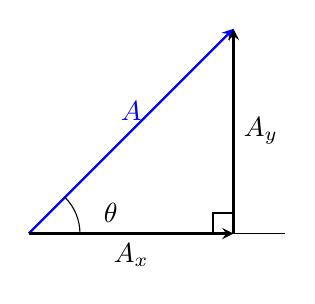
\begin{tikzpicture}[scale=1.3]
        \draw [-stealth, thick, color=blue] (0, 0) -- (2, 2) node [above, midway] {$\va{A}$};
        \draw (0.5, 0) arc(0:45:0.5);
        \node at (0.8, 0.2) {$\theta$};
        \draw (0, 0) -- (2.5, 0);
        \draw [-stealth, thick] (2, 0) -- (2, 2) node [right, midway] {$A_{y}$};
        \draw [-stealth, thick] (0, 0) -- (2, 0) node [below, midway] {$A_{x}$};
        \draw (1.8, 0) -- (1.8, 0.2) -- (2, 0.2);
    \end{tikzpicture}
\end{figure}
El valor del ángulo $\theta$ es:
\pause
\begin{align*}
\theta = \tan \left( \dfrac{A_y}{A_{x}} \right)
\end{align*}
\end{frame}


\section{La geometría necesaria}
\frame{\frametitle{Contenido}\tableofcontents[currentsection, hideothersubsections]}
\subsection{Funciones trigonométricas}

\begin{frame}
\frametitle{El signo de las funciones trigonométricas}
Como estaremos trabajando en los cuatro cuadrantes de un plano cartesiano, es conveniente identificar el signo de la función trigonométrica, ya que nos indicará el valor que habrá que tomar cuando se haga una suma de componentes de varios vectores.
\end{frame}
\begin{frame}
\frametitle{Primer cuadrante}
\begin{figure}
    \centering
    \begin{tikzpicture}
        \begin{tikzpicture}[shift={(1.5, 1)}, scale=1.3]
            \draw (-2, 0) -- (3, 0);
            \draw (0, -1) -- (0, 2.5);
            \draw [-stealth, thick, color=blue] (0, 0) -- (2, 2) node [above, midway] {$\va{A}$};
            \draw (0.5, 0) arc(0:45:0.5);
            \node at (0.8, 0.2) {$\theta$};
            \draw (0, 0) -- (2.5, 0);
            \draw [-stealth, thick] (2, 0) -- (2, 2) node [right, midway] {$A_{y}$};
            \draw [-stealth, thick] (0, 0) -- (2, 0) node [below, midway] {$A_{x}$};
            \draw (1.8, 0) -- (1.8, 0.2) -- (2, 0.2);
        \end{tikzpicture}
    \end{tikzpicture}
\end{figure}
\begin{align*}
A_{y} = \sin \theta \, \abs{A} \hspace{1cm} A_{x} = \cos \theta \, \abs{A} \hspace{1cm} \tan \theta = \dfrac{A_{y}}{A_{x}}
\end{align*}
\end{frame}
\begin{frame}
\frametitle{Segundo cuadrante}
\begin{figure}[H]
    \centering
    \begin{tikzpicture}
        \begin{tikzpicture}[shift={(3.5, 1)}, scale=1.3]
            \draw (-2, 0) -- (0.75, 0);
            \draw (0, -1) -- (0, 2.5);
            \draw [-stealth, thick, color=blue] (0, 0) -- (-2, 2) node [above, midway] {$\va{A}$};
            \draw (0.5, 0) arc(0:135:0.5);
            \node at (0.8, 0.4) {$\theta$};
            \draw (0, 0) -- (0.75, 0);
            \draw [-stealth, thick] (-2, 0) -- (-2, 2) node [left, midway] {$A_{y}$};
            \draw [-stealth, thick] (0, 0) -- (-2, 0) node [below, midway] {$A_{x}$};
            \draw (-1.8, 0) -- (-1.8, 0.2) -- (-2, 0.2);
            \draw [red] (-0.5, 0) arc(180:135:0.5);
            \node at (-0.9, 0.3) {$\alpha$};
        \end{tikzpicture}
    \end{tikzpicture}
\end{figure}
El ángulo $\alpha$ es un ángulo suplementario, por lo que:
\pause
\begin{align*}
\theta = \ang{180} - \alpha
\end{align*}
\end{frame}
\begin{frame}
\frametitle{Segundo cuadrante}
\begin{figure}
    \centering
    \begin{tikzpicture}
        \begin{tikzpicture}[shift={(3.5, 1)}, scale=1.3]
            \draw (-2, 0) -- (0.75, 0);
            \draw (0, -1) -- (0, 2.5);
            \draw [-stealth, thick, color=blue] (0, 0) -- (-2, 2) node [above, midway] {$\va{A}$};
            \draw (0.5, 0) arc(0:135:0.5);
            \node at (0.8, 0.4) {$\theta$};
            \draw (0, 0) -- (0.75, 0);
            \draw [-stealth, thick] (-2, 0) -- (-2, 2) node [left, midway] {$A_{y}$};
            \draw [-stealth, thick] (0, 0) -- (-2, 0) node [below, midway] {$A_{x}$};
            \draw (-1.8, 0) -- (-1.8, 0.2) -- (-2, 0.2);
            \draw [red] (-0.5, 0) arc(180:135:0.5);
            \node at (-0.9, 0.3) {$\alpha$};
        \end{tikzpicture}
    \end{tikzpicture}
\end{figure}
\begin{align*}
A_{y} = \sin \alpha \, \abs{A} \hspace{1cm} A_{x} = - \cos \alpha \, \abs{A}
\end{align*}
\end{frame}
\begin{frame}
\frametitle{Segundo cuadrante}
\begin{figure}
    \centering
    \begin{tikzpicture}
        \begin{tikzpicture}[shift={(3.5, 1)}, scale=1.3]
            \draw (-2, 0) -- (0.75, 0);
            \draw (0, -1) -- (0, 2.5);
            \draw [-stealth, thick, color=blue] (0, 0) -- (-2, 2) node [above, midway] {$\va{A}$};
            \draw (0.5, 0) arc(0:135:0.5);
            \node at (0.8, 0.4) {$\theta$};
            \draw (0, 0) -- (0.75, 0);
            \draw [-stealth, thick] (-2, 0) -- (-2, 2) node [left, midway] {$A_{y}$};
            \draw [-stealth, thick] (0, 0) -- (-2, 0) node [below, midway] {$A_{x}$};
            \draw (-1.8, 0) -- (-1.8, 0.2) -- (-2, 0.2);
            \draw [red] (-0.5, 0) arc(180:135:0.5);
            \node at (-0.9, 0.3) {$\alpha$};
        \end{tikzpicture}
    \end{tikzpicture}
\end{figure}
\begin{align*}
\tan \alpha = - \dfrac{A_{y}}{A_{x}} \hspace{1cm} \theta = \ang{180} - \alpha
\end{align*}
\end{frame}
\begin{frame}
\frametitle{Tercer cuadrante}
\begin{figure}
    \centering
    \begin{tikzpicture}
        \begin{tikzpicture}[shift={(3.5, 2)}, scale=1.3]
            \draw (-2.5, 0) -- (0.75, 0);
            \draw (0, -2.5) -- (0, 1);
            \draw [-stealth, thick, color=blue] (0, 0) -- (-2, -2) node [above, midway] {$\va{A}$};
            \draw (0.5, 0) arc(0:225:0.51);
            \node at (0.8, 0.4) {$\theta$};
            \draw (0, 0) -- (0.75, 0);
            \draw [-stealth, thick] (-0, 0) -- (0, -2) node [right, midway] {$A_{y}$};
            \draw [-stealth, thick] (0, -2) -- (-2, -2) node [below, midway] {$A_{x}$};
            \draw (0, -1.8) -- (-0.2, -1.8) -- (-0.2, -2);
            \draw [red] (0, -0.5) arc(270:225:0.5);
            \node at (-0.3, -0.6) {$\alpha$};
        \end{tikzpicture}
    \end{tikzpicture}
\end{figure}
\vspace*{-2cm}
El ángulo $\alpha$ es complementario en el tercer cuadrante, es decir:
\pause
\begin{align*}
\theta = \ang{270} - \alpha
\end{align*}
\end{frame}
\begin{frame}
\frametitle{Tercer cuadrante}
\begin{figure}
    \centering
    \begin{tikzpicture}
        \begin{tikzpicture}[shift={(3.5, 2)}, scale=1.3]
            \draw (-2.5, 0) -- (0.75, 0);
            \draw (0, -2.5) -- (0, 1);
            \draw [-stealth, thick, color=blue] (0, 0) -- (-2, -2) node [above, midway] {$\va{A}$};
            \draw (0.5, 0) arc(0:225:0.51);
            \node at (0.8, 0.4) {$\theta$};
            \draw (0, 0) -- (0.75, 0);
            \draw [-stealth, thick] (-0, 0) -- (0, -2) node [right, midway] {$A_{y}$};
            \draw [-stealth, thick] (0, -2) -- (-2, -2) node [below, midway] {$A_{x}$};
            \draw (0, -1.8) -- (-0.2, -1.8) -- (-0.2, -2);
            \draw [red] (0, -0.5) arc(270:225:0.5);
            \node at (-0.3, -0.6) {$\alpha$};
        \end{tikzpicture}
    \end{tikzpicture}
\end{figure}
\vspace*{-2cm}
\begin{align*}
A_{y} = -\cos \alpha \, \abs{A} \hspace{1cm} A_{x} = - \sin \alpha \, \abs{A}
\end{align*}
\end{frame}
\begin{frame}
\frametitle{Tercer cuadrante}
\begin{figure}
    \centering
    \begin{tikzpicture}
        \begin{tikzpicture}[shift={(3.5, 2)}, scale=1.3]
            \draw (-2.5, 0) -- (0.75, 0);
            \draw (0, -2.5) -- (0, 1);
            \draw [-stealth, thick, color=blue] (0, 0) -- (-2, -2) node [above, midway] {$\va{A}$};
            \draw (0.5, 0) arc(0:225:0.51);
            \node at (0.8, 0.4) {$\theta$};
            \draw (0, 0) -- (0.75, 0);
            \draw [-stealth, thick] (-0, 0) -- (0, -2) node [right, midway] {$A_{y}$};
            \draw [-stealth, thick] (0, -2) -- (-2, -2) node [below, midway] {$A_{x}$};
            \draw (0, -1.8) -- (-0.2, -1.8) -- (-0.2, -2);
            \draw [red] (0, -0.5) arc(270:225:0.5);
            \node at (-0.3, -0.6) {$\alpha$};
        \end{tikzpicture}
    \end{tikzpicture}
\end{figure}
\vspace*{-2cm}
\begin{align*}
\tan \alpha = - \dfrac{A_{y}}{A_{x}} \hspace{1cm} \theta = \ang{270} - \alpha
\end{align*}    
\end{frame}
\begin{frame}
\frametitle{Cuarto cuadrante}
\begin{figure}
    \centering
    \begin{tikzpicture}
        \begin{tikzpicture}[shift={(1, 2)}, scale=1.3]
            \draw (-1, 0) -- (2.75, 0);
            \draw (0, -2.5) -- (0, 1);
            \draw [-stealth, thick, color=blue] (0, 0) -- (2, -2) node [below, midway] {$\va{A}$};
            \draw (0.5, 0) arc(0:315:0.51);
            \node at (-0.8, 0.4) {$\theta$};
            % \draw (0, 0) -- (0.75, 0);
            \draw [-stealth, thick] (2, 0) -- (2, -2) node [right, midway] {$A_{y}$};
            \draw [-stealth, thick] (0, 0) -- (2, 0) node [above, midway] {$A_{x}$};
            \draw (1.8, 0) -- (1.8, -0.2) -- (2, -0.2);
            \draw [red] (0.5, 0) arc(0:-45:0.5);
            \node at (0.8, -0.4) {$\alpha$};
        \end{tikzpicture}
    \end{tikzpicture}
\end{figure}
\vspace*{-2cm}
El ángulo $\alpha$ es complementario en el cuarto cuadrante, es decir:
\pause
\begin{align*}
\theta = \ang{360} - \alpha
\end{align*}
\end{frame}
\begin{frame}
\frametitle{Cuarto cuadrante}
\begin{figure}
    \centering
    \begin{tikzpicture}
        \begin{tikzpicture}[shift={(1, 2)}, scale=1.3]
            \draw (-1, 0) -- (2.75, 0);
            \draw (0, -2.5) -- (0, 1);
            \draw [-stealth, thick, color=blue] (0, 0) -- (2, -2) node [below, midway] {$\va{A}$};
            \draw (0.5, 0) arc(0:315:0.51);
            \node at (-0.8, 0.4) {$\theta$};
            % \draw (0, 0) -- (0.75, 0);
            \draw [-stealth, thick] (2, 0) -- (2, -2) node [right, midway] {$A_{y}$};
            \draw [-stealth, thick] (0, 0) -- (2, 0) node [above, midway] {$A_{x}$};
            \draw (1.8, 0) -- (1.8, -0.2) -- (2, -0.2);
            \draw [red] (0.5, 0) arc(0:-45:0.5);
            \node at (0.8, -0.4) {$\alpha$};
        \end{tikzpicture}
    \end{tikzpicture}
\end{figure}
\vspace*{-2cm}
\begin{align*}
A_{y} = -\sin \alpha \, \abs{A} \hspace{1cm} A_{x} = \cos \alpha \, \abs{A}
\end{align*}
\end{frame}
\begin{frame}
\frametitle{Cuarto cuadrante}
\begin{figure}
    \centering
    \begin{tikzpicture}
        \begin{tikzpicture}[shift={(1, 2)}, scale=1.3]
            \draw (-1, 0) -- (2.75, 0);
            \draw (0, -2.5) -- (0, 1);
            \draw [-stealth, thick, color=blue] (0, 0) -- (2, -2) node [below, midway] {$\va{A}$};
            \draw (0.5, 0) arc(0:315:0.51);
            \node at (-0.8, 0.4) {$\theta$};
            % \draw (0, 0) -- (0.75, 0);
            \draw [-stealth, thick] (2, 0) -- (2, -2) node [right, midway] {$A_{y}$};
            \draw [-stealth, thick] (0, 0) -- (2, 0) node [above, midway] {$A_{x}$};
            \draw (1.8, 0) -- (1.8, -0.2) -- (2, -0.2);
            \draw [red] (0.5, 0) arc(0:-45:0.5);
            \node at (0.8, -0.4) {$\alpha$};
        \end{tikzpicture}
    \end{tikzpicture}
\end{figure}
\vspace*{-2cm}
\begin{align*}
\tan \alpha = - \dfrac{A_{y}}{A_{x}} \hspace{1cm} \theta = \ang{360} - \alpha
\end{align*}    
\end{frame}

\section{Ejercicio 1}
\frame{\frametitle{Contenido}\tableofcontents[currentsection, hideothersubsections]}
\subsection{Comprobación analítica}

\begin{frame}
\frametitle{Comprobación analítica}
Es posible corroborar el resultado gráfico a partir de la descomposición en componentes de cada uno de los vectores.
\end{frame}
\begin{frame}
\frametitle{Componentes de la resultante}
Llamemos $d_{R}$ el vector resultante de sumar los vectores:
\begin{align*}
d_{R} = d_{1} + d_{2} + d_{3} + d_{4} 
\end{align*}
\pause
Sabemos que en términos de las componentes en $x$, $y$, el vector resultante:
\pause
\begin{align*}
\abs{d_{R}} = \sqrt{(d_{Rx})^{2} + (d_{Ry})^{2}}
\end{align*}
\end{frame}
\begin{frame}
\frametitle{Las componentes}
Y que cada componente está dada por:
\pause
\begin{eqnarray*}
\begin{aligned}
d_{Rx} &= \nsum_{i=1}^{4} d_{ix} \\[0.5em]
d_{Ry} &= \nsum_{i=1}^{4} d_{iy}
\end{aligned}
\end{eqnarray*}
\end{frame}
\begin{frame}
\frametitle{Componentes por vector: $d_{1}$}
Para el vector $d_{1} = \SI{400}{\meter}, \theta = \ang{35}$
\pause
\begin{figure}
    \centering
    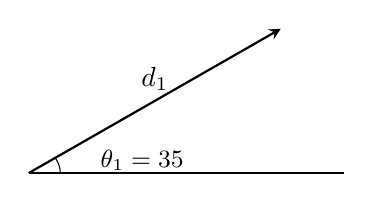
\begin{tikzpicture}[scale=0.8]
        \draw [-stealth, thick] (0, 0) -- (4, 2.29) node [above, midway] {$d_{1}$};
        \draw (0, 0) -- (5, 0);
        \draw (0.5, 0) arc(0:35:0.4);
        \node at (1.8, 0.2) {\small{$\theta_{1} = \ang{35}$}};
    \end{tikzpicture}
\end{figure}
\end{frame}
\begin{frame}
\frametitle{Componentes por vector: $d_{1}$}
\begin{figure}
    \centering
    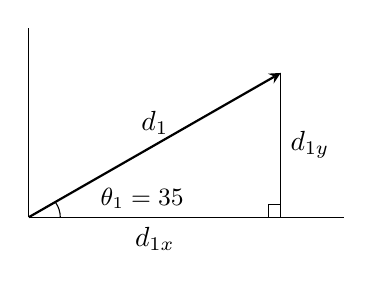
\begin{tikzpicture}[scale=0.8]
        \draw (0, 0) -- (0, 3);
        \draw [-stealth, thick] (0, 0) -- (4, 2.29) node [above, midway] {$d_{1}$};
        \draw (0, 0) -- (5, 0);
        \draw (0.5, 0) arc(0:35:0.4);
        \node at (1.8, 0.3) {\small{$\theta_{1} = \ang{35}$}};
        \draw (3.8, 0) -- (3.8, 0.2) -- (4, 0.2);
        \draw (4, 0) -- (4, 2.29) node [right, midway] {$d_{1y}$};
        \draw (0, 0) -- (4, 0) node [below, midway] {$d_{1x}$};
    \end{tikzpicture}
\end{figure}
\pause
\begin{eqnarray*}
\begin{aligned}
d_{1x} &= \cos \theta \cdot d_{1} = \pause \cos \ang{35} (\SI{400}{\meter}) = \pause \SI{327.66}{\meter} \\[0.5em] \pause
d_{1y} &= \sin \theta \cdot d_{1} = \pause \sin \ang{35} (\SI{400}{\meter}) = \SI{229.43}{\meter}
\end{aligned}
\end{eqnarray*}
\end{frame}
\begin{frame}
\frametitle{Componentes por vector: $d_{2}$}
Para el vector $d_{2} = \SI{700}{\meter}, \theta = \ang{120}$
\pause
\begin{figure}
    \centering
    \begin{tikzpicture}[scale=0.5]
    \draw [-stealth, thick] (4, 2.29) -- (0.5, 8.35) node [midway, right] {$d_{2}$};
            \draw (4, 2.29) -- (5, 2.29);
            \draw (4.5, 2.29) arc(0:120:0.5);
            \node at (5.8, 3.4) {\small{$\theta_{2} = \ang{120}$}};
    \end{tikzpicture}
\end{figure}
\end{frame}
\begin{frame}
\frametitle{Componentes por vector: $d_{2}$}
\begin{figure}
    \centering
    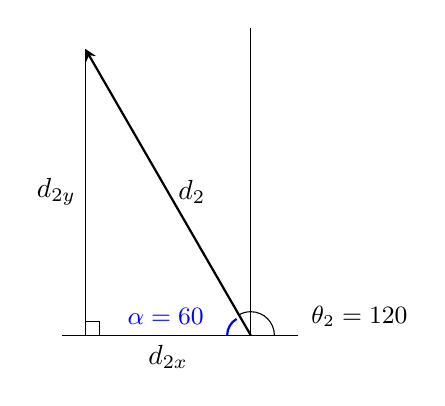
\begin{tikzpicture}[scale=0.6]
        \draw (1, 0) -- (-4, 0);
        \draw (0, 0) --  (0, 6.5);
        \draw [-stealth, thick] (0, 0) -- (-3.5, 6.06) node [midway, right] {$d_{2}$};
        \draw (0.5, 0) arc(0:120:0.5);
        \node at (2.3, 0.4) {\small{$\theta_{2} = \ang{120}$}};
        
        \draw [thick, color=blue] (-0.5, 0) arc(180:120:0.4);
        \node at (-1.8, 0.4) [color=blue] {\small{$\alpha = \ang{60}$}};
        
        \draw (-3.2, 0) -- (-3.2, 0.3) -- (-3.5, 0.3);
        \draw (0, 0) -- (-3.5, 0) node [below, midway] {$d_{2x}$};
        \draw (-3.5, 0) -- (-3.5, 6.06) node [left, midway] {$d_{2y}$};
    \end{tikzpicture}
\end{figure}
\pause
\begin{eqnarray*}
\begin{aligned}
d_{2x} &= -\cos \alpha \cdot d_{2} = \pause-\cos \ang{60} (\SI{700}{\meter}) = \pause -\SI{350}{\meter} \\[0.5em] \pause
d_{2y} &= \sin \alpha \cdot d_{2} = \pause \sin \ang{60} (\SI{700}{\meter}) = \SI{606.21}{\meter}
\end{aligned}
\end{eqnarray*}
\end{frame}    
\begin{frame}
\frametitle{Componentes por vector: $d_{3}$}
Para el vector $d_{3} = \SI{600}{\meter}, \theta = \ang{190}$
\begin{figure}
    \centering
    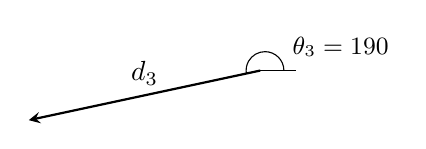
\begin{tikzpicture}[scale=0.6]
        \draw [-stealth, thick] (0.0, 0) -- (-4.9, -1.05) node [above, midway] {$d_{3}$};
        \draw (0, 0) -- (0.75, 0);
        \draw (0.5, 0) arc(0:190:0.4);
        \node at (1.7, 0.5) {\small{$\theta_{3} = \ang{190}$}};
    \end{tikzpicture}
\end{figure}
\end{frame}    
\begin{frame}
\frametitle{Componentes por vector: $d_{3}$}
\begin{figure}
    \centering
    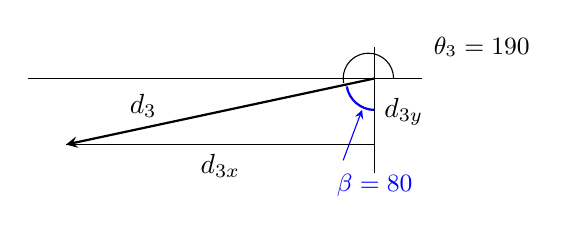
\begin{tikzpicture}[scale=0.8]
        \draw (0, 0) -- (-5.5, 0);
        \draw (0, 0.5) -- (0, -1.5);
        \draw [-stealth, thick] (0.0, 0) -- (-4.9, -1.05) node [above, near end] {$d_{3}$};
        \draw (0, 0) -- (0.75, 0);
        \draw (0.3, 0) arc(0:190:0.4);
        \node at (1.7, 0.5) {\small{$\theta_{3} = \ang{190}$}};
        \draw [blue, thick] (0, -0.5) arc(270:190:0.45);
        \draw [-stealth, color=blue] (-0.5, -1.3) -- (-0.2, -0.5);
        \node at (0, -1.7) [color=blue] {\small{$\beta = \ang{80}$}};
        \draw (0, 0) -- (0, -1.05) node [right, midway] {$d_{3y}$};
        \draw (0, -1.05) -- (-4.9, -1.05) node [below, midway] {$d_{3x}$};
    \end{tikzpicture}
\end{figure}
\begin{eqnarray*}
\begin{aligned}
d_{3x} &= -\sin \beta \cdot d_{3} = \pause -\sin \ang{80} (\SI{600}{\meter}) = \pause -\SI{590.88}{\meter} \\[0.5em] \pause
d_{3y} &= -\cos \beta \cdot d_{3} = \pause -\cos \ang{80} (\SI{600}{\meter}) = -\SI{104.18}{\meter}
\end{aligned}
\end{eqnarray*}
\end{frame}
\begin{frame}
\frametitle{Componentes por vector: $d_{4}$}
Para el vector $d_{4} = \SI{200}{\meter}, \theta = \ang{250}$
\begin{figure}
    \centering
    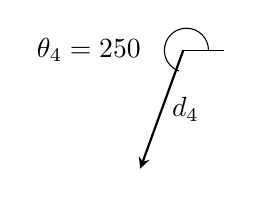
\begin{tikzpicture}[scale=0.8]
        \draw [-stealth, thick] (0, 0) -- (-0.684, -1.879) node [midway, right] {$d_{4}$};
        \draw (0, 0) -- (0.65, 0);
        \draw (0.4, 0) arc(0:250:0.35);
        \node at (-1.5, 0) {$\theta_{4} = \ang{250}$};
    \end{tikzpicture}
\end{figure}
\end{frame}
\begin{frame}
\frametitle{Componentes por vector: $d_{4}$}
\begin{figure}
    \centering
    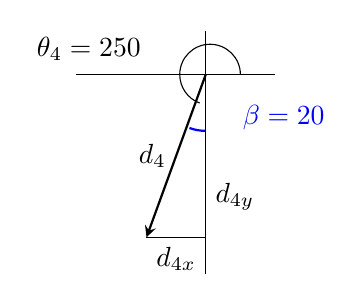
\begin{tikzpicture}[scale=1.1]
        \draw (0.8, 0) -- (-1.5, 0);
        \draw (0, 0.5) -- (0, -2.3);
        \draw [-stealth, thick] (0, 0) -- (-0.684, -1.879) node [midway, left] {$d_{4}$};
        \draw (0, 0) -- (0.65, 0);
        \draw (0.4, 0) arc(0:250:0.35);
        \node at (-1.35, 0.3) {$\theta_{4} = \ang{250}$};

        \draw [color=blue, thick] (0, -0.65) arc(270:250:0.55);
        \node at(0.9, -0.5) [color=blue] {$\beta = \ang{20}$};
        \draw (0, 0) -- (0, -1.879) node [right, near end] {$d_{4y}$};
        \draw (0, -1.879) -- (-0.684, -1.879) node [below, midway] {$d_{4x}$};
    \end{tikzpicture}
\end{figure}
\pause
\begin{eqnarray*}
\begin{aligned}
d_{4x} &= -\sin \beta \cdot h = \pause -\sin \ang{20} (\SI{200}{\meter}) = \pause -\SI{68.40}{\meter} \\[0.5em] \pause
d_{4y} &= -\cos \beta \cdot h = \pause -\cos \ang{20} (\SI{200}{\meter}) = -\SI{187.93}{\meter}
\end{aligned}
\end{eqnarray*}
\end{frame}
\begin{frame}
\frametitle{Sumando las componentes}
Se tiene entonces que:
\pause
\begin{eqnarray*}
\begin{aligned}
&d_{Rx} = \nsum_{i=1}^{4} d_{ix} = \\[0.5em] \pause
&= \SI{327.66}{\meter} {+} (- \SI{350}{\meter}) {+} (- \SI{590.88}{\meter}) {+} (- \SI{68.40}{\meter}) = \\[0.5em] \pause
&= - \SI{681.62}{\meter}
\end{aligned}
\end{eqnarray*}
\end{frame}
\begin{frame}
\frametitle{Sumando las componentes}
Se tiene entonces que:
\pause
\begin{eqnarray*}
\begin{aligned}
&d_{Ry} = \nsum_{i=1}^{4} d_{iy} = \\[0.5em] \pause
&= \SI{229.43}{\meter} {+} (\SI{606.21}{\meter}) {+} (- \SI{104.18}{\meter}) {+} (- \SI{187.93}{\meter}) = \\[0.5em] \pause
&= \SI{540.53}{\meter}
\end{aligned}
\end{eqnarray*}
\end{frame}
\begin{frame}
\frametitle{Del cuadrante del vector resultante}
De las magnitudes de las componentes del vector resultante, es decir, de $d_{Rx}$ y $d_{Ry}$, encontramos el cuadrante en el que se localiza el vector.
\\
\bigskip
\pause
Recordemos que ya teníamos identificado el cuadrante a partir del método gráfico.
\end{frame}
\begin{frame}
\frametitle{Del cuadrante del vector resultante}
Como $d_{Rx}$ tiene una magnitud negativa y $d_{Ry}$ es positiva, \pause sabemos que el vector resultante $d_{R}$ se localiza en el segundo cuadrante.
\\
\bigskip
\pause
Esto nos ayudará para determinar el valor del ángulo $\theta_{R}$.
\end{frame}
\begin{frame}
\frametitle{El vector resultante}
\begin{figure}
    \centering
    \begin{tikzpicture}[scale=0.7]
        \draw (-6.5, 0) -- (1.5, 0);
        \draw (0, 0) -- (0, 6);
        \draw [-stealth, thick, color=blue] (0, 0) -- (-6.084, 5.421) node [midway, above, rotate=-35] {$d_{R}$}; \pause
        \draw [thick, color=blue] (1, 0) arc(0:141.45:0.9);
        \node [blue] at (0.5, 1.4) {$\theta_{R}$};
        \draw (-6.084, 0) -- (-6.084, 5.421) node [left, midway] {$d_{Ry}$};
        \draw (0, 0) -- (-6.084, 0) node [below, midway] {$d_{Rx}$};
        \draw (-5.8, 0) -- (-5.8, 0.3) -- (-6.084, 0.3);
        \draw [color=red, thick] (-1, 0) arc(180:141.58:1);
        \node [red] at (-1.4, 0.3) {$\beta$};
    \end{tikzpicture}
\end{figure}
\end{frame}
\begin{frame}
\frametitle{La magnitud del vector resultante}
La magnitud del vector resultante es:
\pause
\begin{eqnarray*}
\begin{aligned}
\abs{d_{R}} &= \sqrt{(d_{Rx})^{2} + (d_{Ry})^{2}} = \\[0.5em] \pause
&= \sqrt{ (- \SI{681.62}{\meter})^{2} + \SI{540.53}{\meter})^{2}} = \\[0.5em] \pause
&= \sqrt{ \SI{464605.82}{\square\meter} + \SI{292712.68}{\square\meter} } = \\[0.5em] \pause
&= \sqrt{\SI{757318.50}{\square\meter}} = \\[0.5em] \pause
&= \SI{870.24}{\meter}
\end{aligned}
\end{eqnarray*}
\pause
Que es el valor que debemos de anotar como respuesta.
\end{frame}
\begin{frame}
\frametitle{El ángulo de la resultante}
De la trigonometría se obtiene el valor del ángulo auxilar $\beta$ en el segundo cuadrante, \pause y una vez conocido, podremos calcular el valor de $\theta_{R}$ que es el correspondiente al vector resultante:
\pause
\begin{eqnarray*}
\begin{aligned}
\tan \beta &= \dfrac{d_{Ry}}{d_{Rx}} = \pause \dfrac{\SI{540.53}{\meter}}{- \SI{681.62}{\meter}} = \\[0.5em] \pause
\tan \beta &= - 0.7930
\end{aligned}
\end{eqnarray*}
\end{frame}
\begin{frame}
\frametitle{El ángulo de la resultante}
Para recuperar el valor del ángulo, usamos la función inversa, el arco tangente:
\pause
\begin{eqnarray*}
\begin{aligned}
\Rightarrow \arctan(\tan \beta) &= \arctan (-0.7930) = \\[0.5em] \pause
\beta &= - \ang{38.41}
\end{aligned}
\end{eqnarray*}
\end{frame}
\begin{frame}
\frametitle{El ángulo de la resultante}
Como $\beta$ es un ángulo suplementario, \pause podemos obtener el valor de $\theta_{R}$:
\pause
\begin{eqnarray*}
\begin{aligned}
\theta_{R} &= -\alpha + \ang{180} \\[0.5em] \pause
\theta_{R} &= - \ang{38.41} \pause + \ang{180} = \\[0.5em] \pause
\theta_{R} &= \ang{141.58}
\end{aligned}
\end{eqnarray*}
\pause
Esta es la segunda respuesta que nos pide el Ejercicio 1.
\end{frame}
\begin{frame}
\frametitle{El vector resultante}
\begin{figure}
    \centering
    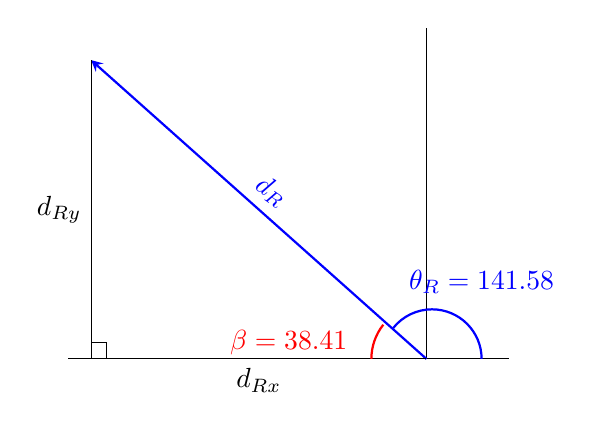
\begin{tikzpicture}[scale=0.7]
        \draw (-6.5, 0) -- (1.5, 0);
        \draw (0, 0) -- (0, 6);
        \draw [-stealth, thick, color=blue] (0, 0) -- (-6.084, 5.421) node [midway, above, rotate=-35] {$d_{R}$}; \pause
        \draw [thick, color=blue] (1, 0) arc(0:141.45:0.9);
        \node [blue] at (1, 1.4) {$\theta_{R} = \ang{141.58}$};
        \draw (-6.084, 0) -- (-6.084, 5.421) node [left, midway] {$d_{Ry}$};
        \draw (0, 0) -- (-6.084, 0) node [below, midway] {$d_{Rx}$};
        \draw (-5.8, 0) -- (-5.8, 0.3) -- (-6.084, 0.3);
        \draw [color=red, thick] (-1, 0) arc(180:141.58:1);
        \node [red] at (-2.5, 0.3) {$\beta = \ang{38.41}$};
    \end{tikzpicture}
\end{figure}
\end{frame}
\begin{frame}
\frametitle{Valores obtenidos}
Con este procedimiento encontramos los valores de la magnitud y dirección del vector resultante, \pause que a diferencia del método gráfico, los valores son más \emph{precisos}, es decir, mejoran los que se recuperaron con el método gráfico.
\end{frame}
\begin{frame}
\frametitle{Del método analítico}
Prácticamente en todo ejercicio que involucre el cálculo de vectores, el método analítico es la manera en la que recuperamos la magnitud y dirección del vector resultante.
\end{frame}

\end{document}